\documentclass[12pt,a4paper]{ctexart}
\setCJKmainfont{Microsoft YaHei}
\usepackage[margin=2.2cm]{geometry}
\usepackage{graphicx}
\usepackage{tikz}
\usetikzlibrary{positioning}
\newcommand{\pk}[1]{\texttt{#1}}
\newcommand{\fk}[1]{\textcolor{gray}{\texttt{#1}}}
\usepackage{enumitem}
\usepackage{hyperref}
\usepackage{listings}
\usepackage{xcolor}

\hypersetup{colorlinks=true,linkcolor=blue,urlcolor=blue}

\lstset{
  basicstyle=\small\ttfamily,
  backgroundcolor=\color{gray!10},
  frame=single,
  breaklines=true,
  language=SQL
}

\title{\textbf{SQL 判题考试系统 —— 项目文档}}
\author{第三组}
\date{\today}

\begin{document}

\maketitle
\tableofcontents
\newpage

% ===================================================================
\section{系统需求分析}
% ===================================================================

\subsection{项目背景}

数据库课程（如 CS304 / DB304）的教学过程中，SQL 练习和考试是两个核心环节。传统方式下，学生提交 SQL 作业后需要教师手动批改，考试也需要人工阅卷，效率低且反馈周期长。本项目旨在构建一个在线 SQL 判题与考试系统，实现 SQL 练习的自动判题、在线考试的自动评分，以及班级和成绩的统一管理。

\subsection{用户角色}

系统定义四类用户角色，采用最小权限原则：

\begin{description}[leftmargin=2em]
  \item[学生（STUDENT）] 浏览题库、编写 SQL 练习、参加在线考试、查看个人提交记录和成绩。
  \item[教师（TEACHER）] 创建和管理班级、维护题库和测试用例、创建和发布考试、查看学生提交和班级成绩统计。
  \item[管理员（ADMIN）] 用户增删改查、角色分配、账号状态管理、系统全局数据查看。
  \item[助教（ASSISTANT）] 预留角色，MVP 阶段尚未细化授权，当前可查看提交记录和成绩统计。
\end{description}

\subsection{功能需求}

\begin{enumerate}[leftmargin=2em]
  \item \textbf{用户认证}：注册、登录、JWT 鉴权、密码修改。注册接口已锁定，新用户由管理员创建。
  \item \textbf{题库管理}：教师创建/编辑/删除题目，支持 Markdown 题面、表结构展示、难度分级、标签分类。学生浏览和搜索题目。
  \item \textbf{SQL 判题}：学生在 Monaco Editor 中编写 SQL，支持运行自测和正式提交。系统自动执行判题，返回 AC/WA/ERROR/TLE/FORBIDDEN 状态。
  \item \textbf{在线考试}：教师通过四步向导创建考试（配置参数 → 选题 → 设分值 → 分配学生），发布后学生在指定时间窗口内作答。支持多题导航、独立草稿、自动交卷。
  \item \textbf{班级管理}：教师创建班级并生成邀请码，学生通过邀请码加入班级。
  \item \textbf{成绩统计}：教师查看考试成绩排名、平均分、最高分。成绩由服务端自动汇总每题最高分，不可前端篡改。
  \item \textbf{用户管理}：管理员创建/编辑用户，调整角色和账号状态。
  \item \textbf{仪表盘}：学生端展示已解决题目数、正确率、连续练习天数、即将考试、推荐题目。教师端展示班级数、题库量、待处理提交、最近考试。
\end{enumerate}

% ===================================================================
\section{数据库设计}
% ===================================================================

\subsection{概念模型（E-R 图）}

系统包含 9 张核心数据表，实体关系如下：

\begin{center}
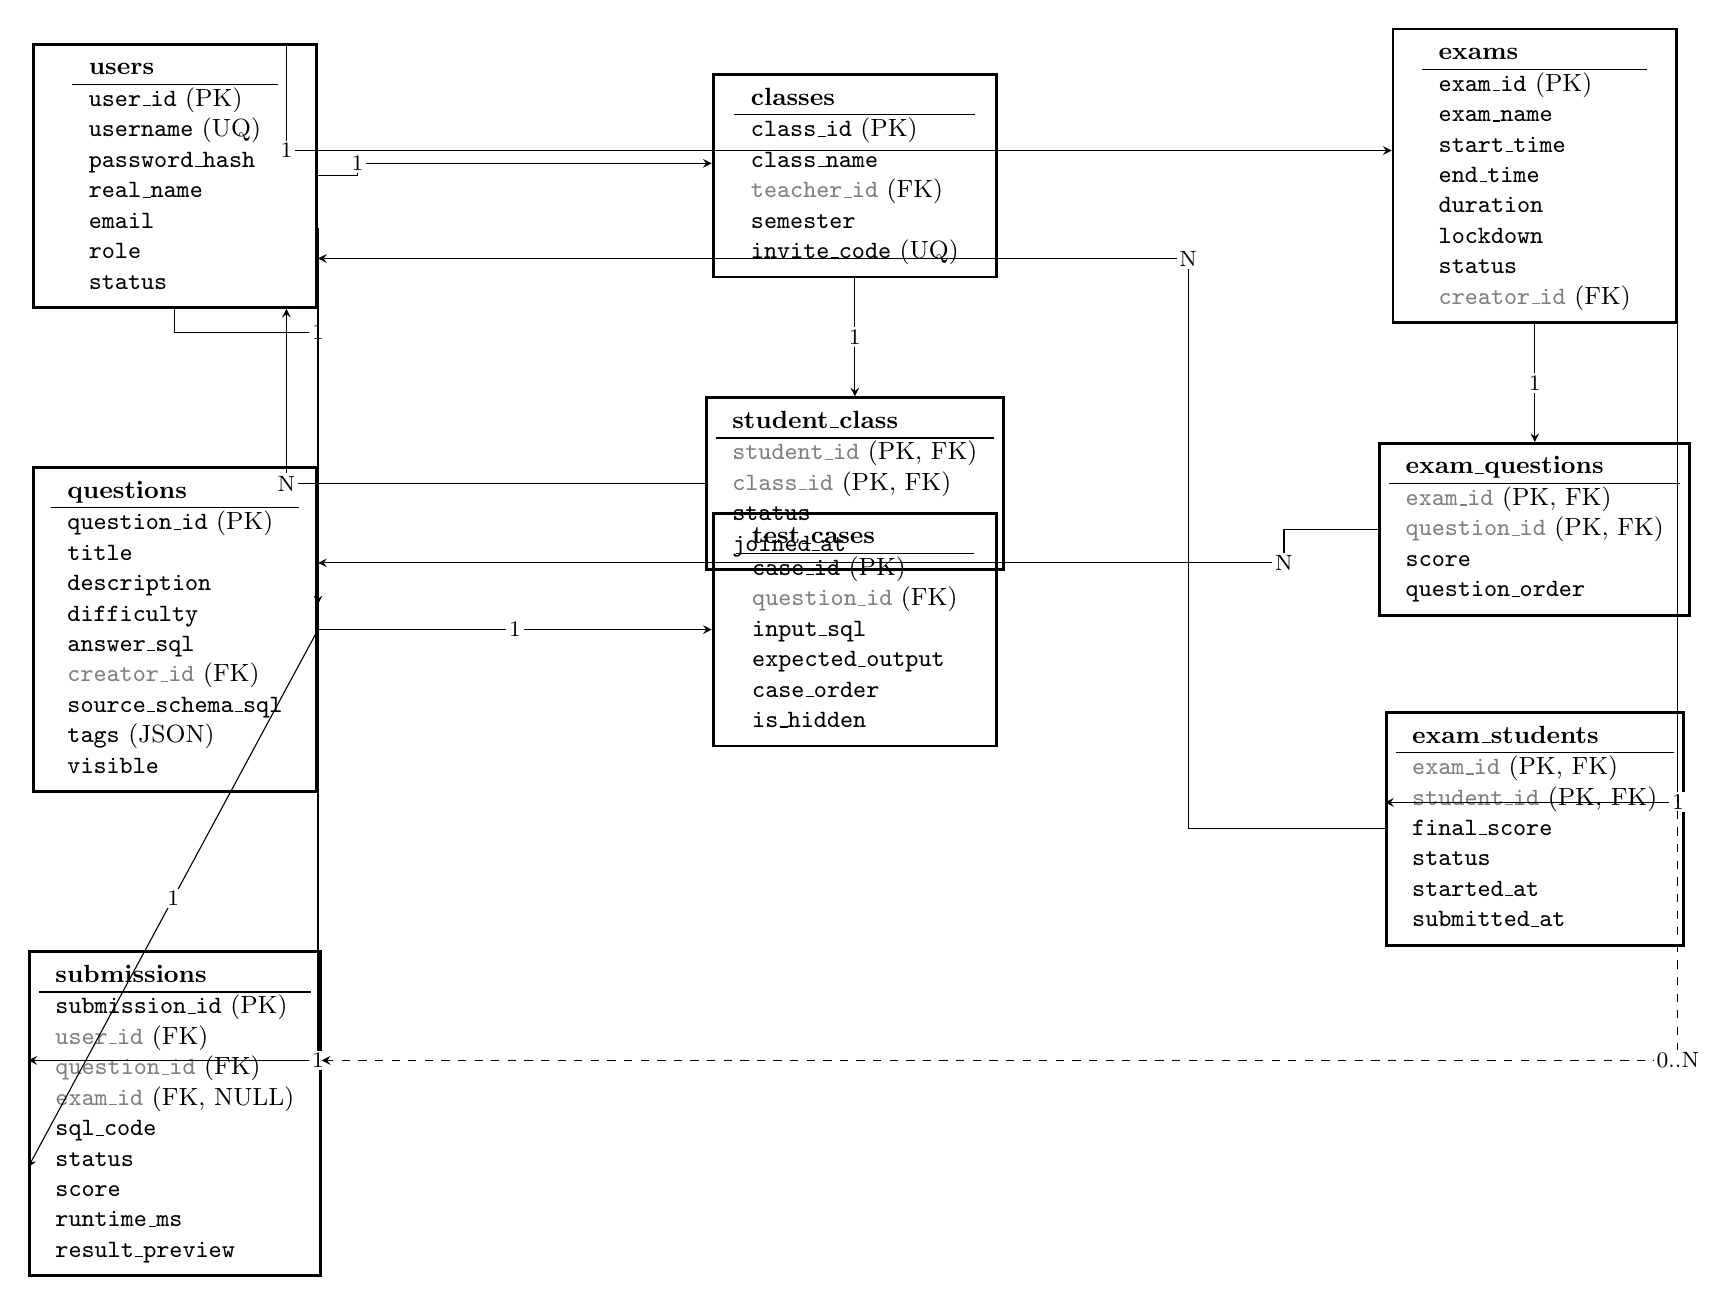
\begin{tikzpicture}[
    node distance=2.8cm and 3.2cm,
    table/.style={rectangle,draw=black,line width=1pt,minimum width=3.6cm,font=\small},
    pk/.style={font=\small\ttfamily},
    fk/.style={font=\small\ttfamily,text=black!60},
    rel/.style={font=\footnotesize,midway,fill=white,inner sep=1pt},
    >=stealth
  ]
  \node[table] (users) at (0,0) {%
    \begin{tabular}{l}
      \textbf{users} \\ \hline
      \pk{user\_id} (PK) \\
      \texttt{username} (UQ) \\
      \texttt{password\_hash} \\
      \texttt{real\_name} \\
      \texttt{email} \\
      \texttt{role} \\
      \texttt{status} \\
    \end{tabular}
  };
  \node[table,right=5cm of users] (classes) {%
    \begin{tabular}{l}
      \textbf{classes} \\ \hline
      \pk{class\_id} (PK) \\
      \texttt{class\_name} \\
      \fk{teacher\_id} (FK) \\
      \texttt{semester} \\
      \texttt{invite\_code} (UQ) \\
    \end{tabular}
  };
  \node[table,below=2cm of users] (questions) {%
    \begin{tabular}{l}
      \textbf{questions} \\ \hline
      \pk{question\_id} (PK) \\
      \texttt{title} \\
      \texttt{description} \\
      \texttt{difficulty} \\
      \texttt{answer\_sql} \\
      \fk{creator\_id} (FK) \\
      \texttt{source\_schema\_sql} \\
      \texttt{tags} (JSON) \\
      \texttt{visible} \\
    \end{tabular}
  };
  \node[table,right=5cm of questions] (test_cases) {%
    \begin{tabular}{l}
      \textbf{test\_cases} \\ \hline
      \pk{case\_id} (PK) \\
      \fk{question\_id} (FK) \\
      \texttt{input\_sql} \\
      \texttt{expected\_output} \\
      \texttt{case\_order} \\
      \texttt{is\_hidden} \\
    \end{tabular}
  };
  \node[table,right=5cm of classes] (exams) {%
    \begin{tabular}{l}
      \textbf{exams} \\ \hline
      \pk{exam\_id} (PK) \\
      \texttt{exam\_name} \\
      \texttt{start\_time} \\
      \texttt{end\_time} \\
      \texttt{duration} \\
      \texttt{lockdown} \\
      \texttt{status} \\
      \fk{creator\_id} (FK) \\
    \end{tabular}
  };
  \node[table,below=2cm of questions] (submissions) {%
    \begin{tabular}{l}
      \textbf{submissions} \\ \hline
      \pk{submission\_id} (PK) \\
      \fk{user\_id} (FK) \\
      \fk{question\_id} (FK) \\
      \fk{exam\_id} (FK, NULL) \\
      \texttt{sql\_code} \\
      \texttt{status} \\
      \texttt{score} \\
      \texttt{runtime\_ms} \\
      \texttt{result\_preview} \\
    \end{tabular}
  };
  \node[table,below=1.5cm of classes] (student_class) {%
    \begin{tabular}{l}
      \textbf{student\_class} \\ \hline
      \fk{student\_id} (PK, FK) \\
      \fk{class\_id} (PK, FK) \\
      \texttt{status} \\
      \texttt{joined\_at} \\
    \end{tabular}
  };
  \node[table,below=1.5cm of exams] (exam_questions) {%
    \begin{tabular}{l}
      \textbf{exam\_questions} \\ \hline
      \fk{exam\_id} (PK, FK) \\
      \fk{question\_id} (PK, FK) \\
      \texttt{score} \\
      \texttt{question\_order} \\
    \end{tabular}
  };
  \node[table,below=1.2cm of exam_questions] (exam_students) {%
    \begin{tabular}{l}
      \textbf{exam\_students} \\ \hline
      \fk{exam\_id} (PK, FK) \\
      \fk{student\_id} (PK, FK) \\
      \texttt{final\_score} \\
      \texttt{status} \\
      \texttt{started\_at} \\
      \texttt{submitted\_at} \\
    \end{tabular}
  };

  % Relations
  \draw[->] (users.east) -- ++(0.5,0) |- node[rel] {1} (classes.175);
  \draw[->] (users.south) -- ++(0,-0.3) -| node[rel] {1} (questions.10);
  \draw[->] (users.50) |- node[rel] {1} (exams.170);
  \draw[->] (users.340) |- node[rel] {1} (submissions.160);
  \draw[->] (classes.south) -- (student_class.north) node[rel] {1};
  \draw[->] (student_class.west) -| node[rel] {N} (users.310);
  \draw[->] (questions.east) -- node[rel] {1} (test_cases.west);
  \draw[->] (questions.0) -- node[rel] {1} (submissions.200);
  \draw[->] (exams.south) -- (exam_questions.north) node[rel] {1};
  \draw[->] (exam_questions.west) -| ++(-1.2,0) |- node[rel] {N} (questions.25);
  \draw[->] (exams.355) |- node[rel] {1} (exam_students.170);
  \draw[->] (exam_students.west) -| ++(-2.5,0) |- node[rel] {N} (users.330);
  \draw[->,dashed] (exams.5) |- node[rel] {0..N} (submissions.20);
\end{tikzpicture}
\end{center}

\subsection{物理模型（DDL）}

共 9 张表，使用 InnoDB 引擎，utf8mb4 字符集。外键统一采用 \texttt{ON DELETE RESTRICT ON UPDATE RESTRICT}，防止误删造成历史数据丢失。

\subsubsection*{users —— 用户表}

\begin{lstlisting}[language=SQL]
CREATE TABLE users (
  user_id       BIGINT PRIMARY KEY AUTO_INCREMENT,
  username      VARCHAR(64) NOT NULL,
  password_hash VARCHAR(255) NOT NULL,
  real_name     VARCHAR(64),
  email         VARCHAR(128),
  role          ENUM('STUDENT','TEACHER','ADMIN','ASSISTANT') NOT NULL,
  status        ENUM('ACTIVE','DISABLED') NOT NULL DEFAULT 'ACTIVE',
  created_at    DATETIME NOT NULL DEFAULT CURRENT_TIMESTAMP,
  updated_at    DATETIME NOT NULL DEFAULT CURRENT_TIMESTAMP ON UPDATE CURRENT_TIMESTAMP,
  UNIQUE KEY uk_users_username (username),
  UNIQUE KEY uk_users_email (email)
) ENGINE=InnoDB;
\end{lstlisting}

\subsubsection*{classes —— 班级表}

\begin{lstlisting}[language=SQL]
CREATE TABLE classes (
  class_id    BIGINT PRIMARY KEY AUTO_INCREMENT,
  class_name  VARCHAR(128) NOT NULL,
  teacher_id  BIGINT NOT NULL,
  semester    VARCHAR(64),
  invite_code VARCHAR(32),
  created_at  DATETIME NOT NULL DEFAULT CURRENT_TIMESTAMP,
  updated_at  DATETIME NOT NULL DEFAULT CURRENT_TIMESTAMP ON UPDATE CURRENT_TIMESTAMP,
  UNIQUE KEY uk_classes_invite_code (invite_code),
  FOREIGN KEY (teacher_id) REFERENCES users(user_id)
    ON DELETE RESTRICT ON UPDATE RESTRICT
) ENGINE=InnoDB;
\end{lstlisting}

\subsubsection*{student\_class —— 学生班级关联表}

\begin{lstlisting}[language=SQL]
CREATE TABLE student_class (
  student_id BIGINT NOT NULL,
  class_id   BIGINT NOT NULL,
  status     ENUM('ACTIVE','PENDING','REMOVED') NOT NULL DEFAULT 'ACTIVE',
  joined_at  DATETIME NOT NULL DEFAULT CURRENT_TIMESTAMP,
  PRIMARY KEY (student_id, class_id),
  FOREIGN KEY (student_id) REFERENCES users(user_id)
    ON DELETE RESTRICT ON UPDATE RESTRICT,
  FOREIGN KEY (class_id) REFERENCES classes(class_id)
    ON DELETE RESTRICT ON UPDATE RESTRICT
) ENGINE=InnoDB;
\end{lstlisting}

\subsubsection*{questions —— 题目表}

\begin{lstlisting}[language=SQL]
CREATE TABLE questions (
  question_id       BIGINT PRIMARY KEY AUTO_INCREMENT,
  title             VARCHAR(200) NOT NULL,
  description       MEDIUMTEXT NOT NULL,
  difficulty        ENUM('EASY','MEDIUM','HARD') NOT NULL DEFAULT 'MEDIUM',
  answer_sql        MEDIUMTEXT NOT NULL,
  creator_id        BIGINT NOT NULL,
  source_schema_sql MEDIUMTEXT,
  tags              JSON,
  visible           TINYINT(1) NOT NULL DEFAULT 1,
  created_at        DATETIME NOT NULL DEFAULT CURRENT_TIMESTAMP,
  updated_at        DATETIME NOT NULL DEFAULT CURRENT_TIMESTAMP ON UPDATE CURRENT_TIMESTAMP,
  INDEX idx_questions_difficulty (difficulty),
  FOREIGN KEY (creator_id) REFERENCES users(user_id)
    ON DELETE RESTRICT ON UPDATE RESTRICT
) ENGINE=InnoDB;
\end{lstlisting}

\subsubsection*{test\_cases —— 测试用例表}

\begin{lstlisting}[language=SQL]
CREATE TABLE test_cases (
  case_id         BIGINT PRIMARY KEY AUTO_INCREMENT,
  question_id     BIGINT NOT NULL,
  input_sql       MEDIUMTEXT NOT NULL,
  expected_output JSON NOT NULL,
  case_order      INT NOT NULL DEFAULT 1,
  is_hidden       TINYINT(1) NOT NULL DEFAULT 0,
  created_at      DATETIME NOT NULL DEFAULT CURRENT_TIMESTAMP,
  FOREIGN KEY (question_id) REFERENCES questions(question_id)
    ON DELETE RESTRICT ON UPDATE RESTRICT
) ENGINE=InnoDB;
\end{lstlisting}

\subsubsection*{exams —— 考试表}

\begin{lstlisting}[language=SQL]
CREATE TABLE exams (
  exam_id          BIGINT PRIMARY KEY AUTO_INCREMENT,
  exam_name        VARCHAR(200) NOT NULL,
  start_time       DATETIME NOT NULL,
  end_time         DATETIME NOT NULL,
  duration_minutes INT,
  instructions     MEDIUMTEXT,
  lockdown_enabled TINYINT(1) NOT NULL DEFAULT 0,
  status           ENUM('DRAFT','PUBLISHED','FINISHED','ARCHIVED')
                     NOT NULL DEFAULT 'DRAFT',
  creator_id       BIGINT NOT NULL,
  created_at       DATETIME NOT NULL DEFAULT CURRENT_TIMESTAMP,
  updated_at       DATETIME NOT NULL DEFAULT CURRENT_TIMESTAMP ON UPDATE CURRENT_TIMESTAMP,
  CONSTRAINT ck_exams_time CHECK (end_time > start_time),
  CONSTRAINT ck_exams_duration CHECK (duration_minutes IS NULL OR duration_minutes > 0),
  FOREIGN KEY (creator_id) REFERENCES users(user_id)
    ON DELETE RESTRICT ON UPDATE RESTRICT
) ENGINE=InnoDB;
\end{lstlisting}

\subsubsection*{exam\_questions —— 考试题目关联表}

\begin{lstlisting}[language=SQL]
CREATE TABLE exam_questions (
  exam_id        BIGINT NOT NULL,
  question_id    BIGINT NOT NULL,
  score          DECIMAL(5,2) NOT NULL,
  question_order INT NOT NULL DEFAULT 1,
  PRIMARY KEY (exam_id, question_id),
  CONSTRAINT ck_exam_questions_score CHECK (score >= 0 AND score <= 100),
  FOREIGN KEY (exam_id) REFERENCES exams(exam_id)
    ON DELETE RESTRICT ON UPDATE RESTRICT,
  FOREIGN KEY (question_id) REFERENCES questions(question_id)
    ON DELETE RESTRICT ON UPDATE RESTRICT
) ENGINE=InnoDB;
\end{lstlisting}

\subsubsection*{exam\_students —— 考试学生关联表}

\begin{lstlisting}[language=SQL]
CREATE TABLE exam_students (
  exam_id      BIGINT NOT NULL,
  student_id   BIGINT NOT NULL,
  final_score  DECIMAL(6,2) NOT NULL DEFAULT 0,
  status       ENUM('NOT_STARTED','ONGOING','SUBMITTED','ABSENT')
                 NOT NULL DEFAULT 'NOT_STARTED',
  started_at   DATETIME,
  submitted_at DATETIME,
  PRIMARY KEY (exam_id, student_id),
  CONSTRAINT ck_exam_students_score CHECK (final_score >= 0),
  FOREIGN KEY (exam_id) REFERENCES exams(exam_id)
    ON DELETE RESTRICT ON UPDATE RESTRICT,
  FOREIGN KEY (student_id) REFERENCES users(user_id)
    ON DELETE RESTRICT ON UPDATE RESTRICT
) ENGINE=InnoDB;
\end{lstlisting}

\subsubsection*{submissions —— 提交记录表}

\begin{lstlisting}[language=SQL]
CREATE TABLE submissions (
  submission_id BIGINT PRIMARY KEY AUTO_INCREMENT,
  user_id       BIGINT NOT NULL,
  question_id   BIGINT NOT NULL,
  exam_id       BIGINT,
  sql_code      MEDIUMTEXT NOT NULL,
  status        ENUM('PENDING','AC','WA','ERROR','TLE','FORBIDDEN')
                  NOT NULL DEFAULT 'PENDING',
  score         DECIMAL(6,2) NOT NULL DEFAULT 0,
  runtime_ms    INT,
  memory_kb     INT,
  error_message TEXT,
  result_preview JSON,
  submit_time   DATETIME NOT NULL DEFAULT CURRENT_TIMESTAMP,
  CONSTRAINT ck_submissions_score CHECK (score >= 0),
  INDEX idx_submissions_user_time (user_id, submit_time),
  INDEX idx_submissions_exam_user (exam_id, user_id),
  FOREIGN KEY (user_id) REFERENCES users(user_id)
    ON DELETE RESTRICT ON UPDATE RESTRICT,
  FOREIGN KEY (question_id) REFERENCES questions(question_id)
    ON DELETE RESTRICT ON UPDATE RESTRICT,
  FOREIGN KEY (exam_id) REFERENCES exams(exam_id)
    ON DELETE RESTRICT ON UPDATE RESTRICT
) ENGINE=InnoDB;
\end{lstlisting}

\subsection{关键设计说明}

\begin{enumerate}[leftmargin=2em]
  \item \texttt{questions.description} 使用 Markdown 格式存储题面，前端渲染为安全 HTML。
  \item \texttt{test\_cases.expected\_output} 使用 JSON 格式存储期望结果，结构为 \texttt{\{"columns":[], "rows":[[]], "orderSensitive": false\}}。数字类型做规范化比较（\texttt{1} 与 \texttt{1.0} 视为相等），NULL 严格匹配。
  \item \texttt{submissions.exam\_id} 可为 NULL。为 NULL 表示日常练习，不为 NULL 表示考试提交。
  \item 题目采用软删除（\texttt{visible = 0}）而非物理删除，保留历史提交记录的外键关联。
  \item \texttt{exam\_students.final\_score} 由服务端按各题最高分汇总写入，前端不可直接传值。
  \item 所有外键使用 \texttt{ON DELETE RESTRICT}，防止级联删除破坏数据完整性。
\end{enumerate}

% ===================================================================
\section{判题引擎设计}
% ===================================================================

\subsection{判题范围（MVP）}

第一版只支持查询类 SQL 语句：

\begin{itemize}
  \item \textbf{允许}：SELECT、WITH（CTE）、JOIN、GROUP BY、HAVING、子查询、窗口函数等。
  \item \textbf{禁止}：INSERT、UPDATE、DELETE、DROP、ALTER、CREATE、TRUNCATE、GRANT、REVOKE、CALL、LOAD DATA，以及任何形式的多语句执行。
\end{itemize}

后续如需支持 DML 类题目，需要单独扩展执行策略和结果比对方式。

\subsection{三层安全防护}

\subsubsection*{第一层：关键字黑名单}

在 SQL 字符串层面检查是否包含禁止的关键字：DROP、INSERT、UPDATE、DELETE、ALTER、CREATE、TRUNCATE、GRANT、REVOKE、CALL。命中任一关键字直接返回 FORBIDDEN。

\subsubsection*{第二层：分号计数}

统计 SQL 字符串中分号的数量。通过比较首个分号和末个分号的字符串位置来判断：如果首尾分号位置不同，说明存在多个分号即多语句，拒绝执行。字符串常量内部的分号不会被计入。

\subsubsection*{第三层：JSqlParser AST 解析}

将 SQL 字符串解析为抽象语法树（AST），校验根节点必须是 \texttt{Select} → \texttt{PlainSelect}。如果是 \texttt{SetOperationList}（UNION / INTERSECT / EXCEPT）或包含 DML 子句，直接拒绝。

引入 JSqlParser 的关键原因是：关键字黑名单和分号计数都属于字符串级防护，无法应对语法层面的绕过。例如 UNION 查询可以组合两个合法 SELECT 来间接获取数据，只有 AST 级别的节点类型判断才能从根本上拦截这类攻击。

\subsection{执行流程}

\begin{enumerate}[leftmargin=2em]
  \item 前端提交 SQL → 系统创建 \texttt{submissions} 记录（\texttt{status = PENDING}）。
  \item 加载题目信息、测试用例、考试题目分值（如为考试提交）。
  \item SQL 安全检查（三层防护）。
  \item 对每个测试用例执行以下步骤：
  \begin{enumerate}
    \item 创建临时 MySQL Schema，命名格式为 \texttt{judge\_\{questionId\}\_\{timestamp\}\_\{uuid\}}。
    \item 执行测试用例的 \texttt{input\_sql} 初始化表和数据。
    \item 使用低权限 MySQL 账号执行学生 SQL，设置 \texttt{maxExecutionTime} = 5 秒。
    \item 读取结果集，转为规范化 JSON 格式。
    \item 与 \texttt{expected\_output} 逐项比对。
    \item 在 \texttt{finally} 块中删除临时 Schema。
  \end{enumerate}
  \item 汇总所有测试用例的通过情况，计算得分。
  \item 更新 \texttt{submissions} 记录（status、score、runtime\_ms、error\_message、result\_preview）。
  \item 若为考试提交，触发最终成绩重算。
\end{enumerate}

\subsection{结果比对规则}

\begin{enumerate}[leftmargin=2em]
  \item 列名必须匹配，默认不区分大小写。
  \item 列数量必须一致。
  \item 行数量必须一致。
  \item 若 \texttt{orderSensitive = false}，将双方行按整行 JSON 字符串排序后比较。
  \item 数字类型规范化：\texttt{1} 与 \texttt{1.0} 视为相等。
  \item NULL 必须与 NULL 匹配，不与空字符串混淆。
  \item 字符串精确匹配，不做内部空格 trim。
\end{enumerate}

\subsection{安全策略总结}

\begin{enumerate}[leftmargin=2em]
  \item 判题 MySQL 用户仅拥有临时 Schema 下的权限，不拥有业务库 \texttt{sql\_exam} 的任何权限。
  \item 每次执行使用独立 JDBC 连接，设置语句超时。
  \item JDBC 连接禁用 \texttt{allowMultiQueries=true}。
  \item SQL 提交前做语法级检查：关键字黑名单 → 分号计数 → JSqlParser AST 解析。
  \item 单次查询限制返回最多 1000 行。
  \item 判题失败也必须清理临时 Schema，清理逻辑放在 \texttt{finally} 块中保证执行。
  \item 测试用例的初始化 SQL 只能由教师创建，学生不可编辑。
\end{enumerate}

% ===================================================================
\section{模块划分与系统实现}
% ===================================================================

\subsection{技术栈}

\begin{table}[h]
\centering
\begin{tabular}{lll}
\hline
层次 & 技术 & 说明 \\
\hline
后端框架 & Spring Boot 2.7 + Java 11 & RESTful API，事务管理 \\
ORM/SQL  & MyBatis 2.3.2 & 注解式 SQL 映射，参数化查询 \\
鉴权     & JWT + Spring Security & HMAC-SHA256 签名，BCrypt 密码加密 \\
数据库   & MySQL 8.x & 业务库 \texttt{sql\_exam} + 判题临时 Schema \\
迁移     & Flyway 9.22.3 & 4 个迁移脚本，版本化管理表结构和种子数据 \\
SQL 解析 & JSqlParser 4.9 & AST 语法树解析，安全校验 \\
API 文档 & Springdoc OpenAPI & Swagger UI 自动生成 \\
\hline
前端框架 & Vue 3.4 + TypeScript & Composition API，\texttt{<script setup>} \\
构建     & Vite 5.4 & 开发热更新，生产构建 \\
状态管理 & Pinia 2.1 & Auth Store 管理登录态 \\
路由     & Vue Router 4.3 & 16 条路由，角色级导航守卫 \\
HTTP     & Axios 1.6 & JWT 拦截器，401 自动跳转登录 \\
样式     & Tailwind CSS 3.4 & 自定义设计令牌（颜色、字体、间距） \\
编辑器   & Monaco Editor & SQL 语法高亮、自动补全、快捷键 \\
\hline
\end{tabular}
\end{table}

\subsection{后端模块划分}

后端共 55 个 Java 文件，约 2300 行代码，分为 8 个业务模块和 2 个基础设施包。

\begin{description}[leftmargin=2em,style=nextline]

\item[common 包（5 文件 / 169 行）]
统一响应封装（\texttt{ApiResponse}）、自定义业务异常（\texttt{BusinessException}，错误码 40000--51000）、全局异常处理（\texttt{GlobalExceptionHandler}）、当前用户工具类（\texttt{CurrentUser}）、分页响应（\texttt{PageResponse}）。

\item[security 包（5 文件 / 264 行）]
Spring Security 无状态配置（\texttt{SecurityConfig}）：禁用 Session、启用 CORS、放行登录注册接口、其余接口需 JWT 认证。JWT 生成与解析（\texttt{JwtTokenProvider}）：HMAC-SHA256 签名，包含 userId 和 role。JWT 过滤器（\texttt{JwtAuthenticationFilter}）：从 Authorization Header 提取 Bearer Token，注入 SecurityContext。用户详情服务（\texttt{SqlUserDetailsService}）和 UserPrincipal 实现 UserDetails 接口。

\item[auth 模块（6 文件 / 172 行）]
登录：验证用户名密码，返回 JWT Token 和用户信息。密码修改：校验旧密码正确性、新密码长度、新旧密码不同。注册接口已锁定（返回 403），新用户由管理员创建。

\item[admin 模块（5 文件 / 152 行）]
管理员专属。用户列表查询、创建用户（设置角色和初始密码）、编辑用户（修改角色和状态）。所有接口标注 \texttt{@PreAuthorize("hasRole('ADMIN')")}。

\item[question 模块（9 文件 / 329 行）]
题库完整 CRUD。创建/编辑/软删除题目（\texttt{visible = 0}）。搜索支持关键词同时匹配标题和描述，支持难度筛选，服务端分页。测试用例管理：增删改查，\texttt{expected\_output} 以 JSON 格式存储。权限控制：学生只看到 \texttt{visible = 1} 的题目，答案和测试用例字段在学生返回中为 null。

\item[judge 模块（8 文件 / 453 行）]
系统核心。\texttt{JudgeService}（269 行）：三层安全检查 → 临时 Schema 创建 → 测试用例初始化 → 学生 SQL 执行 → 结果比对 → Schema 清理。\texttt{SubmissionService}：提交记录管理、历史查询、考试成绩触发重算。两个接口：\texttt{run}（自测不存记录）和 \texttt{submit}（正式提交存记录）。

\item[exam 模块（6 文件 / 406 行）]
考试全生命周期管理。创建草稿 → 四步向导配置（参数/选题/分值/分配学生）→ 发布 → 学生作答 → 成绩汇总。\texttt{ExamService}（214 行）：发布状态校验（已发布不可再次发布，已归档不可操作）、学生/题目存在性校验、重复添加检测。成绩重算：取每道题最高提交分，按 \texttt{exam\_questions.score} 上限汇总，写入 \texttt{exam\_students.final\_score}。

\item[classes 模块（5 文件 / 154 行）]
班级 CRUD。教师创建班级时自动生成 8 位随机邀请码。学生通过邀请码加入班级，插入 \texttt{student\_class} 记录。教师调用加入接口返回 403。

\item[dashboard 模块（2 文件 / 116 行）]
学生仪表盘：已解题目数（日常练习不同题目 AC 数）、正确率（总 AC / 总提交）、连续练习天数（AC 提交日期去重后倒推连续天数）、即将考试列表、推荐题目。教师仪表盘：活跃班级数、题库总量、待处理提交（ERROR / FORBIDDEN 状态）、最近考试列表。

\item[user 模块（3 文件 / 90 行）]
用户实体（\texttt{UserRecord}）、数据访问（\texttt{UserMapper}）、种子用户初始化（\texttt{SeedUserInitializer} —— 启动时检查并确保三个默认账号存在，密码使用 BCrypt 哈希）。

\end{description}

\subsection{前端模块划分}

前端共 23 个 Vue 文件，约 2350 行代码（含 TypeScript）。

\subsubsection*{核心基础设施}

\begin{itemize}
  \item \texttt{api/http.ts}：Axios 实例封装，请求拦截器自动添加 JWT Bearer Token，响应拦截器拦截 401 自动跳转登录页。
  \item \texttt{stores/auth.ts}：Pinia Auth Store，管理 token 和 user 状态。\texttt{login()} 调接口存 token 到 localStorage，\texttt{fetchMe()} 获取当前用户信息，\texttt{logout()} 清除状态跳转登录页，页面刷新时从 localStorage 恢复登录态。
  \item \texttt{router/index.ts}：16 条路由，按角色分三级——公开路由（/login）、学生路由（/student/*）、教师路由（/teacher/*）、管理员路由（/admin/*）。路由守卫检查 Pinia auth store 的角色字段，学生访问教师路由自动重定向到学生仪表盘，反之同理。未登录访问任何受保护路由都重定向 /login。
\end{itemize}

\subsubsection*{组件（9 个）}

\begin{itemize}
  \item \texttt{AppLayout.vue}（223 行）：全局布局，包含侧边导航栏（按角色动态渲染菜单）、顶部搜索栏（回车跳转题库搜索）、设置面板（修改密码弹窗）。
  \item \texttt{SqlEditor.vue}（57 行）：Monaco Editor 封装，\texttt{v-model} 双向绑定 SQL 代码，注册 MySQL 语言支持。
  \item \texttt{StatCard.vue}（29 行）：仪表盘统计卡片，展示图标、标签、数值、副标题。
  \item \texttt{ProgressRing.vue}（42 行）：环形进度条组件，用于展示正确率等百分比指标。
  \item \texttt{BarChart.vue}（30 行）：柱状图组件，用于教师端统计展示。
  \item \texttt{WelcomeBanner.vue}、\texttt{ProblemCard.vue}、\texttt{ExamCard.vue}、\texttt{ActivityFeed.vue}：辅助展示组件。
\end{itemize}

\subsubsection*{页面路由表（16 条）}

\begin{table}[h]
\centering
\begin{tabular}{lll}
\hline
路由 & 页面 & 角色 \\
\hline
\texttt{/login}                              & LoginView          & 公开 \\
\texttt{/problems}                           & QuestionList       & 登录 \\
\texttt{/problems/:id}                       & QuestionViewer     & 登录 \\
\texttt{/student/dashboard}                  & StudentDashboard   & 学生 \\
\texttt{/student/submissions}                & StudentSubmissions & 学生 \\
\texttt{/student/exams}                      & StudentExams       & 学生 \\
\texttt{/student/exams/:id/take}             & ExamTake           & 学生 \\
\texttt{/student/classes}                    & StudentClasses     & 学生 \\
\texttt{/teacher/dashboard}                  & TeacherDashboard   & 教师 \\
\texttt{/teacher/questions}                  & TeacherQuestions   & 教师 \\
\texttt{/teacher/classes}                    & TeacherClasses     & 教师 \\
\texttt{/teacher/exams/new}                  & ExamWizard         & 教师 \\
\texttt{/teacher/scores}                     & TeacherScores      & 教师 \\
\texttt{/admin/users}                        & AdminUsers         & 管理员 \\
\hline
\end{tabular}
\end{table}

\subsection{核心技术实现}

\subsubsection*{JWT 鉴权流程}

\begin{enumerate}[leftmargin=2em]
  \item 用户提交用户名密码 → 后端查询 \texttt{users} 表 → BCrypt 比对密码哈希 → 生成 JWT Token（包含 userId、role，HMAC-SHA256 签名，过期时间可配置）。
  \item 前端收到 Token 存入 localStorage 和 Pinia store。
  \item 后续请求在 Authorization Header 中携带 \texttt{Bearer <token>}。
  \item 后端 \texttt{JwtAuthenticationFilter} 从请求中提取 Token → 解析验证 → 注入 SecurityContext → 后续 \texttt{@PreAuthorize} 注解基于角色鉴权。
\end{enumerate}

\subsubsection*{判题引擎核心实现}

\texttt{JudgeService.java}（269 行）是系统最核心的文件，关键实现如下：

\textbf{安全检查（extractSelectBody 方法）：} 调用 JSqlParser 解析 SQL → 获取 \texttt{PlainSelect} 对象。若解析失败（语法错误）→ 返回 null，由外层判定为 ERROR。若解析成功但根节点不是 \texttt{PlainSelect}（如 \texttt{SetOperationList}）→ 返回 null，判定为 FORBIDDEN。

\textbf{临时 Schema 执行（judge 方法）：} 创建 JDBC 连接 → \texttt{CREATE DATABASE judge\_xxx} → \texttt{USE judge\_xxx} → 执行测试用例 \texttt{input\_sql}（CREATE TABLE + INSERT）→ 设置 \texttt{maxExecutionTime} → 执行学生 SQL → 读取 \texttt{ResultSet} → 转为规范化 JSON → 与 \texttt{expected\_output} 比对 → 在 \texttt{finally} 块中 \texttt{DROP DATABASE judge\_xxx}。

\textbf{结果比对（compareResults 方法）：} 逐一检查列名、列数、行数。根据 \texttt{orderSensitive} 决定是否排序后比较。NULL 值特殊处理，数字类型用 \texttt{BigDecimal} 比较。

\subsubsection*{考试成绩重算}

每次考试提交成功后，调用 \texttt{ExamService.recalculateFinalScore(examId, studentId)}：查询该学生在该考试每题的最高提交分 → 按 \texttt{exam\_questions.score} 上限截断 → 求和 → 更新 \texttt{exam\_students.final\_score}。

% ===================================================================
\section{系统安装使用说明}
% ===================================================================

\subsection{环境要求}

\begin{table}[h]
\centering
\begin{tabular}{ll}
\hline
依赖 & 版本要求 \\
\hline
Java  & 11 及以上 \\
MySQL & 8.x 及以上 \\
Node.js & 20 或 22 LTS（不建议 Node 25） \\
Maven  & 内置 Maven Wrapper，无需额外安装 \\
\hline
\end{tabular}
\end{table}

\subsection{一键启动（推荐）}

首次使用需先初始化数据库：

\begin{lstlisting}[language=bash]
DB_USERNAME=root DB_PASSWORD='你的密码' ./start.sh --setup
\end{lstlisting}

启动系统：

\begin{lstlisting}[language=bash]
DB_USERNAME=root DB_PASSWORD='你的密码' ./start.sh
\end{lstlisting}

启动成功后访问：

\begin{itemize}
  \item 前端页面：\texttt{http://localhost:5173}
  \item 登录页：\texttt{http://localhost:5173/login}
  \item 后端 API：\texttt{http://localhost:8080/api}
  \item Swagger 文档：\texttt{http://localhost:8080/swagger-ui.html}
\end{itemize}

停止服务：

\begin{lstlisting}[language=bash]
DB_USERNAME=root DB_PASSWORD='你的密码' ./start.sh --stop
\end{lstlisting}

也可直接在启动终端按 \texttt{Ctrl+C}。

\subsection{手动启动}

\subsubsection*{后端}

\begin{lstlisting}[language=bash]
cd backend
DB_USERNAME=root DB_PASSWORD='你的密码' ./mvnw -DskipTests package
DB_USERNAME=root DB_PASSWORD='你的密码' java -Dfile.encoding=UTF-8 -jar target/exam-0.0.1-SNAPSHOT.jar
\end{lstlisting}

\subsubsection*{前端}

\begin{lstlisting}[language=bash]
cd frontend
npm ci --cache /tmp/sqljudge-npm-cache --no-audit --no-fund
npm run dev -- --host 127.0.0.1 --port 5173 --strictPort
\end{lstlisting}

\subsection{环境变量}

\begin{table}[h]
\centering
\begin{tabular}{lll}
\hline
变量 & 默认值 & 说明 \\
\hline
\texttt{DB\_HOST}     & localhost  & MySQL 主机 \\
\texttt{DB\_PORT}     & 3306       & MySQL 端口 \\
\texttt{DB\_NAME}     & sql\_exam   & 业务库名 \\
\texttt{DB\_USERNAME} & root       & MySQL 用户名 \\
\texttt{DB\_PASSWORD} & —          & MySQL 密码（必填） \\
\texttt{SERVER\_PORT} & 8080       & 后端端口 \\
\texttt{FRONTEND\_PORT}& 5173      & 前端端口 \\
\texttt{JWT\_SECRET}  & —          & JWT 签名密钥 \\
\hline
\end{tabular}
\end{table}

\subsection{默认账号}

\begin{table}[h]
\centering
\begin{tabular}{lll}
\hline
用户名 & 密码 & 角色 \\
\hline
\texttt{admin}    & \texttt{password} & 管理员 \\
\texttt{teacher1} & \texttt{password} & 教师 \\
\texttt{student1} & \texttt{password} & 学生 \\
\hline
\end{tabular}
\end{table}

首次启动时 Flyway 自动执行 4 个迁移脚本：V1 建表 → V2 种子用户 → V3 密码 BCrypt 修正 → V4 导入 10 道 LeetCode 题目。

\subsection{题库数据}

系统预置了 10 道 LeetCode 数据库题目（题号 175--185），包含完整的题面、表结构、参考答案和测试用例。其中 177 原题为函数题，当前平台只允许 SELECT，因此导入为固定 \texttt{N = 2} 的练习版本。

\subsection{常见问题}

\begin{description}[leftmargin=2em,style=nextline]

\item[端口被占用]
查端口占用：\texttt{lsof -nP -iTCP:8080 -sTCP:LISTEN}。若是本项目的残留进程，执行 \texttt{./start.sh --stop} 清理。

\item[前端启动超时]
确认 Node 为 LTS 版本（\texttt{node -v}），然后删除 \texttt{node\_modules} 和 \texttt{package-lock.json} 重新安装。

\item[Maven 打包异常]
清理构建缓存：\texttt{rm -rf backend/target}，然后 \texttt{cd backend \&\& ./mvnw -q -DskipTests package}。

\item[MySQL 连接失败]
确认 MySQL 已启动，并传入正确的用户名密码：\texttt{DB\_USERNAME=root DB\_PASSWORD='你的密码' ./start.sh}。

\item[.pids 目录残留]
删除临时目录后重启：\texttt{rm -rf .pids \&\& ./start.sh}。

\end{description}

\end{document}
